\chapter{Les complexes}
% - Rappels sur les ensembles, introduction des ensembles N et R et notation $x \in A$
% - Rappels sur la valeur absolue, distance et inégalité triangulaire

On définit l'ensemble des nombres complexes par : $i^2 = -1$. Cet ensemble est très pratique, car il nous permet de résoudre des équations de type : $x^2 = -3$ qui est non résoluble dans les réels !

Regardons de plus près les concepts principaux de l'analyse complexe :

\section{Fonction complexes}

On dit qu'une fonction 'f' est complexe, si elle est sous la forme suivante : 
$$f(x,y)= u(x,y) + iv(x,y)$$
dans ce cas de figure, on voit clairement que f nécessite deux variables en entrée pour être opérationnelle, à savoir x et y. De la même façon que f va toujours donner en sortie deux valeurs distinctes, une selon i et l'autre sans. On dira que f est une fonction qui par de $R^2$ vers $R^2$ (noté $R^2 \rightarrow R^2$). Ainsi, ce qui rend l'étude des complexes fondamentalement non intuitive, c'est par ce que la fonction requiert quatre dimensions spatiales pour s'exprimer.

les fonctions u et v sont à eux des fonctions réelles qui peuvent, ou non, dépendre de x et y. Mais elles ne sont pas complexes. Elles prennent deux valeurs en entrée, x et y, mais ne donnent qu'une seule valeur de sortie (on note mathématiquement qu'elles sont ($R^2 \rightarrow R$).

En guise d'exemple, on pourrait prendre la fonction suivante : 
$$f(x,y) = x^2 - 3 + i(y - x + 5)$$
Par identification, on voit clairement ici que : 

$$u(x,y) = x^2 - 3 \text{    et   } v(x,y) = y - x + 5$$ 

Si on décide d'évaluer cette fonction en x = 2 et y = 3, on obtient :

$$f(2,3) = 2^2 - 3 +i(3 - 2 + 5) = 4 - 3 + i6 = 1 + 6i$$

Cet exemple illustre bien la nécessité de définir f comme une fonction $R^2 \rightarrow R^2$, elle a pris deux valeurs distinctes en entrée et a recraché deux valeurs distinctes en sorties, qui sont différenciées par le i.

Cette différenciation entre la partie réelle (qui n'est pas attaché à i) et la partie imaginaire (qui est attaché à i) peut-être exploiter afin de rendre notre écriture encore plus intuitive. Les notations suivantes sont toutes équivalentes : 

$$f(2,3) = f(2 + 3i)$$

\subsection{Coordonnées polaires}


Étant donné que nous avons constamment une distinction nette entre l'axe des abscisses et l'axe des ordonnées (x,y) par l'artifice du i. On peut représenter une coordonnée dans l'univers complexe de plusieurs façons, passons les en revues : 

Coordonnées cartésiennes : 

La notation que nous avons introduite jusqu'à présent est dite cartésienne. On la représente de façon suivante, avec $x_p = 2$ et $y_p = 3$. 

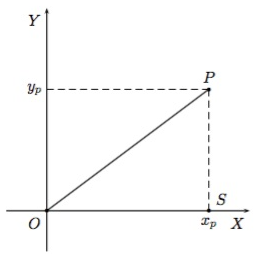
\includegraphics[scale=.5]{assets/imgs/complexe.png}

Coordonnées polaires :

Une autre façon de se représenter un point dans un espace en deux dimensions, c'est de visualiser le mouvement, non pas comme une évolution le long des coordonnées cartésiennes respectives, par exemple le point (2,3) qui va aller vers (4,3) puis vers (4,7). Une première translation selon x a été faite, puis une seconde le long des ordonnées en y jusqu'à aboutir à la position finale.

On peut observer le mouvement sous une autre forme, lors de cette translation, le point s'est nettement éloigné de l'origine du repère, sa distance entre son emplacement original et final a changé ! En polaire, cette distance est dite radiale (du mot rayon), et on notera cette distance $\rho$. Par la même occasion, ce point en question a changé de coordonnée y, passant de 3 à 7, il est donc monté dans le repère. On peut représenter cette montée mathématiquement par la variation d'un angle qui a augmenté en valeur par rapport à l'axe horizontal. On notera cet angle $\theta$.

Nous aboutissons à un nouveau système de coordonnées, tout autant suffisant pour décrire l'emplacement du point que les coordonnées cartésiennes, sous la forme : $(\rho, \theta)$

$$z = x + iy =  \rho(\cos \phi + i\sin \phi) = \rho e^{i\phi}$$

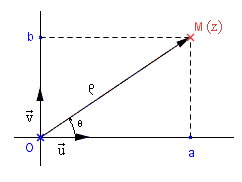
\includegraphics[scale=.5]{assets/imgs/complexe2.png}

\subsection{Rappel notion trigonométrique}

Pour conclure ce bref chapitre, et après avoir rendu compte que les complexes ne sont pas qu'un simple fantasme imaginaire chez les mathématiciens, mais une forme d'analyse à part entière. On vous propose de vous rafraichir la mémoire avec quelques rappels essentiels à fin de pouvoir manipuler l'univers complexe avec aisance, et cela ne peut se faire sans avoir recours à la trigonométrie !

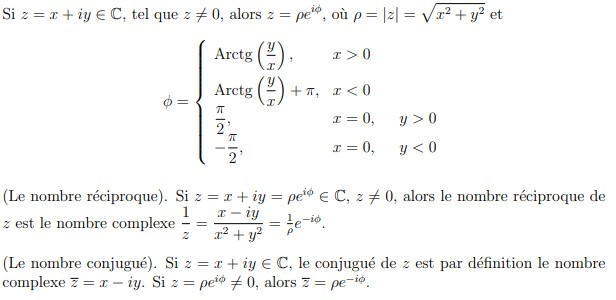
\includegraphics[scale=.7]{assets/imgs/complexe3.jpg}
\newline
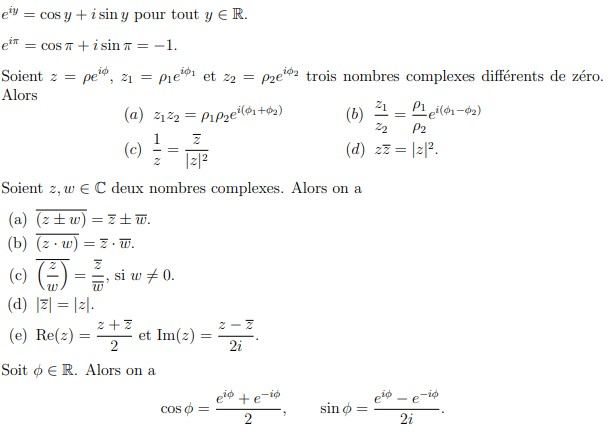
\includegraphics[scale=.7]{assets/imgs/complexe4.jpg}

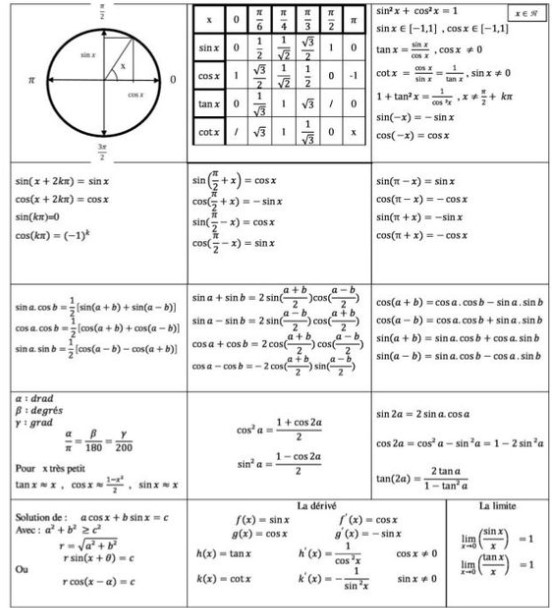
\includegraphics[scale=.8]{assets/imgs/complexe5.jpg}



